

\section{Tervezés}

\subsection{Bevezető}

Ebben a részben elsőként leírom, illetve összehasonlítom a multimédia üzenetküldő rendszer megvalósítási lehetőségeit, majd az általam kiválasztott módszer funkcionális egységeit, azok szerepét és egymással való kapcsolatát részleteiben tárgyalom.

\subsection{A megvalósítási lehetőségek}

Nézzük meg, hogy az IMS használata esetén milyen lehetőségek vannak a csoportos üzenetküldés megvalósítására. A megoldási lehetőségek ismertetése során kitérek azok előnyeire, a hátrányaira, illetve a felmerülő problémákra.

\subsubsection{SIP MESSAGE üzenetek használata}
\label{sec:sip_message}

Első megoldásként kézenfekvőnek tűnhet, hogy a SIP protokoll által nyújtott MESSAGE típusú üzenet törzsében küldjük el a multimédia üzenetet a címzetteknek. Ennek a megoldásnak az az előnye, hogy nem kell másik protokollt használni az üzenetek átviteléért, hanem a SIP protokoll nyújtotta funkciókat alkalmazzuk. A megoldás előnye viszont eltörpül a hátrányok mellett. Először is a MESSAGE típusú üzenetnek nem adható meg egynél több címzett, így minden címzettnek különálló MESSAGE üzenetben kellene elküldeni ugyanazt a tartalmat. Ez a megszorítás redundanciához vezet, mivel a feladónak ugyanazt az üzenetet minden címzettnek külön el kell küldenie, ami a válaszidőt is jelentősen megnöveli. Erre a problémára megoldást jelenthet, ha az üzenetet egy alkalmazás szerveren keresztül küldjük, és ez a szerver továbbítaná azt a címzetteknek. Ebben az esetben a küldő csak egyszer küldené el az üzenetet. Ahhoz, hogy ez a megvalósítás működhessen, a felhasználókból csoportokat kell létrehozni, és a MESSAGE üzenetet a címzettek URI-ja (Uniform Resource Identifier) helyett a csoport URI-jával címezni. Amikor az alkalmazás szerver megkapja ezt az üzenetet, a csoport azonosító alapján megkeresi azokat a felhasználókat, akik tagjai a csoportnak, és mindegyik csoporttagnak egyesével elküldi a kapott üzenet másolatát. Ebben az esetben szükség van az alkalmazás szerver oldalán egy olyan funkcióra, ami a csoportkezelést megvalósítja.
További problémát jelent, ha küldött multimédia mérete meghaladja a MESSAGE üzenet törzsébe maximálisan megadható 1300 oktetet\footnote{RFC 3428 - Session Initiation Protocol Extension for Instant Messaging}. Ilyenkor a tartalmat a küldő oldalon kisebb darabokra kell tördelni, a darabokat külön üzenetekben elküldeni, majd a vevő oldalon a kisebb részekből a teljes üzenetet rekonstruálni. A probléma gyökere, hogy a MESSAGE üzenettípus nem támogatja egy üzenet több darabban való átvitelét. A MESSAGE üzenet fejlécében nincs lehetőség olyan paramétert megadni, amiből a vevő el tudja dönteni, hogy a beérkező MESSAGE üzenetek közül melyik hordozza ugyanazon tartalom egy-egy darabját, és melyik nem, ebből következően rekonstruálni sem tudja azt. További gond, hogy az üzenetek nem sorszámozottak, így azt eredeti küldési sorrendet sem tudnánk visszaállítani. Ezek a problémák abból fakadnak, hogy a MESSAGE üzenet használatát elsősorban rövid szöveges üzenetek továbbítására találták ki -- ami belefér egyetlen üzenetbe --, és nem nagy multimédia tartalmak továbbítására. 
A megoldás hátrányainak sorát bővíti az is, hogy nem támogatott a késleltetett üzenetküldést sem. Utóbbi problémát -- hasonlóan a többszörös küldéshez -- orvosolhatnánk az alkalmazás szerver használatával, amely eltárolná azokat az üzeneteket, amelyek a nem elérhető címzetteknek mennek, és akkor kézbesítené azt, amikor a címzett elérhetővé válik.

{\color{red}(IDE MÉG RFC3428-ból PÁR DOLOG)
(Leírni még, hogy a vevők válasza többször jön, stb...)}

\subsubsection{Több címzettel rendelkező üzenetek használata}
Mint ahogy a \ref{sec:sip_message}.~fejezetben láthattuk, az alap SIP specifikáció nem nyújt hatékony megoldást a több címzettű üzenetek továbbítására. Ebben az alpontban leírt megoldás abban tér el az előzőhöz képest, hogy az üzenet fejlécben lehetőség van több címzettet megadni. A folytatásban az ilyen típusú üzenetet több címzettel rendelkező, azaz MR (Multi Recipient) üzenetnek fogom nevezni. A több címzett megadásának a lehetősége jelentős előnyt jelent az alap SIP MESSAGE-et használó megoldáshoz képest. Először is, a feladónak elég csak egyszer elküldeni az üzenetet a CSCF felé, és nem annyiszor, ahány címzettje van az üzenetnek. Ez jelentősen lecsökkenti a hálózati erőforrások használatát. Másodszor, mivel a címzettek a MR üzenet fejlécében helyezkednek el, így az erre alkalmas hálózati szerverek a fejléc adatokat felhasználva képesek az üzenetek hatékonyan eljuttatni az összes címzettnek anélkül, hogy az üzenet törzsét meg kellene vizsgálniuk. Tegyük fel, hogy a feladó hálózatában lévő S-CSCF, miután megkapja feladótól az MR üzenetet, annak minden címzettjére meghatározza az adott címzett felé vezető következő állomást (next hop CSCF), ahová továbbítani kell azt. Abban az esetben, ha kettő vagy több címzett esetén ugyanaz a next hop, akkor az S-CSCF abba az irányba MR üzenetként küldi tovább az üzenetet. Ha minden címzett next hop CSCF-je különbözik egymástól, akkor a szerver az egyes next hop-oknak hagyományos üzenetben küldi el annak egy-egy másolatát. Mivel hálózatban található összes CSCF hasonlóan viselkedik, mint a feladót kiszolgáló S-CSCF, ezzel a módszerrel két szerver között ugyanaz az üzenet pontosan egyszer kerül átvitelre. Az üzenet terjedésének folyamatát a \ref{fig:mrflow}.~ábrán követhetjük nyomon. Jól látható, hogy ezzel a módszerre minden linken kizárólag egyszer küldjük át ugyanazt az üzenetet, ellentétben az aktuális IMS javaslattal, miszerint több címzett esetén egy linken többször kellene átküldeni ugyanazt az üzenetet (Például a III-as, IV-es és V-ös linken). Abban az esetben, ha egy olyan CSCF vesz egy MR üzenetet, amely nem képes MR üzeneteket kezelni, akkor a küldő CSCF felé hibaüzenetet küld. Ilyenkor a küldő CSCF újra elküldi az üzenetet hagyományos SIP üzenetként, minden címzettre külön-külön.

{\color{red}(Leírni még, hogy a vevők válasza többször jönne, de ez csökkenthető ha az S-CSCF bevár több választ és egybe rakja MR-ként stb...)}
\begin{figure}[htbp]
\center
\resizebox{10cm}{!}{
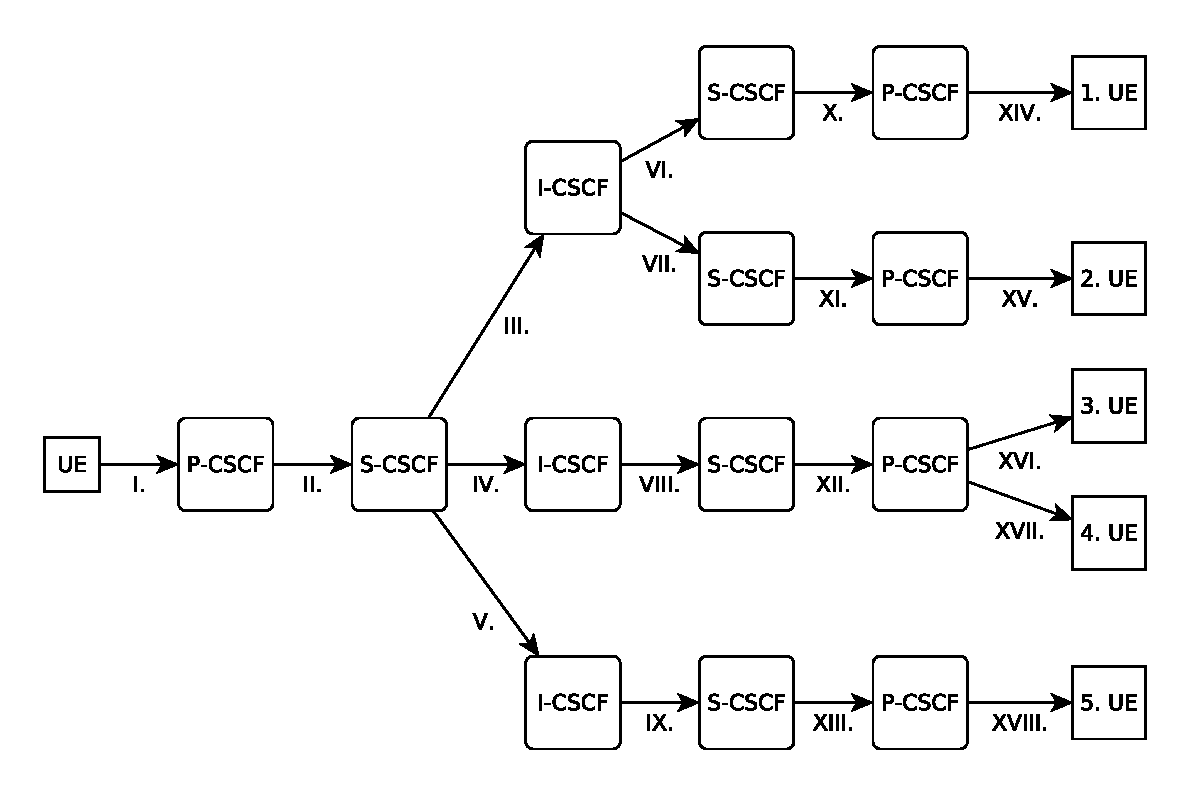
\includegraphics{img/MR-flow.eps}}
\caption{Az MR üzenetküldés folyamata}
\label{fig:mrflow}
\end{figure}

\subsubsection{Üzenet továbbítása RTP protokoll segítségével}
Ide kell MRF, AS stb... Leírni! Ábra? előny, hátrány...

\subsubsection{Üzenet továbbítása MSRP protokollal}
Ezt csinálom én. Először INVITE--OK--ACK üzenetváltással felépíteni a sessiont (SDP-vel leírva), és azon keresztül küldeni az üzenetet. Leírni!! \\
\\
\\
{\color{red}Utóbbira esett a választás jellegű dolog leírása pár mondatban!}

\subsection{Funkcionális terv}

A rendszer a kliens-szerver architektúra szerint épül fel....

\begin{figure}[htbp]
\center
\resizebox{10cm}{!}{
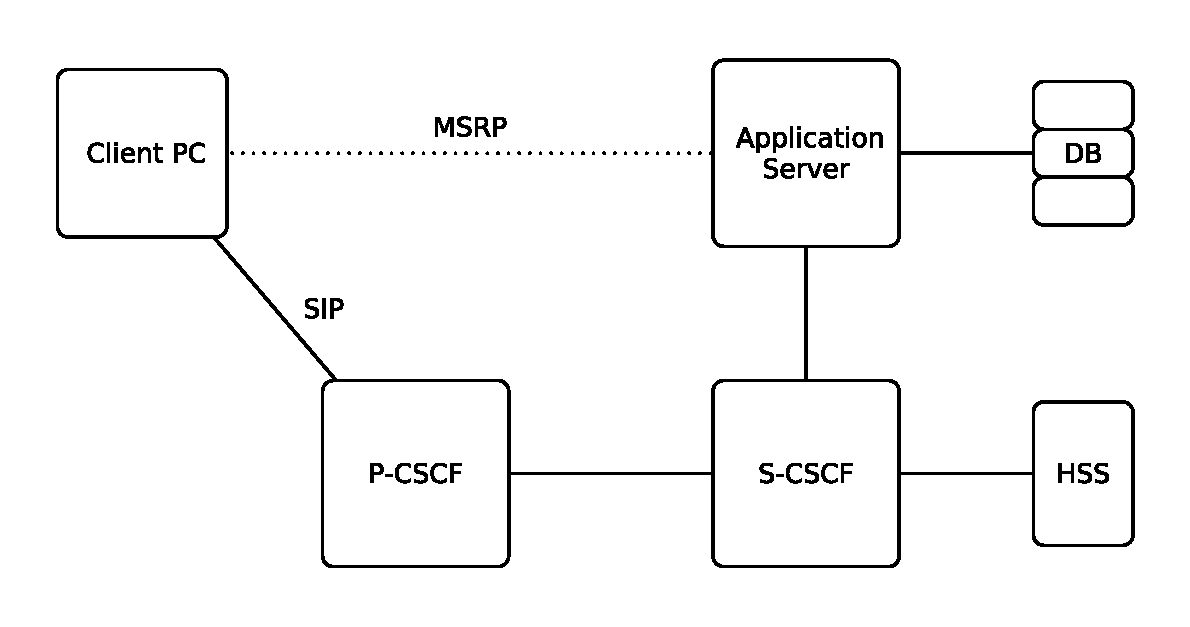
\includegraphics{img/system_MSRP_black.eps}}
\caption{A rendszer magasszintű modellje}
\label{fig:model}
\end{figure}

A következő fejezetekben az egyes elemek funkciójának részletes tárgyalása következik.

\subsubsection{Kliens}
\label{sec:kliens_pc}


\subsubsection{Alkalmazás szerver}
A megvalósítandó üzenetküldő rendszerben központi szerephet jut az alkalmazás szerver, ő végzi az üzenetek címzettenek való szétosztását. A küldő kliens minden esetben az alkalmazás szerverrel építi fel a kapcsolatot, és annak küldi el a multimédia üzenetet. Két felhasználó közvetlenül soha nem küld egymásnak semmit. Az szerver feladata kettős. Egyrészt fogadja a feladótól érkező multimédia üzenetet és továbbítja azt minden címzettnek külön-külön, másrészt a késletetett üzenettovábbítást valósítja meg. Utóbbi funkcióra akkor van szükség, ha a címzettek közül valamelyik nem elérhető. Ebben az esetben az AS akkor küldi el az üzenetet a címzettnek, amikor az elérhetővé válik.

\subsubsection{Adatbázis szerver}
\label{sec:adatbszerver}

A küldő felhasználótól az alkalmazás szerveren keresztül érkező üzenetek átmeneti tárolását valósítja meg. Abban az esetben, ha a címzett felhasználó 

Tárolásra kerülnek a felhasználótól érkező üzenet adatai. Ezek közé tartozik
a feladó azonosítója (SIP URI), a címzettek azonosítói (SIP URI), valamint maga a multimédia üzenet.

\subsubsection{Proxy CSCF}
\label{sec:p_cscf}

\subsubsection{Serving CSCF}
\label{sec:s_cscf}

\subsubsection{HSS}
\label{sec:hss}

\subsection{Tesztelési terv ez nem ide, majd a végére}
\label{sec:tesztelesi_terv}

A rendszer tervezésének fontos részét képezi a funkcionális tesztelés. Leegyszerűsíti a megvalósítást ill. segít elkerülni olyan hibákat, melyekre az imp\-le\-men\-tá\-lás során talán nem derülne fény. A rendszer étékelésének alapjául szolgál.

Teszteket érdemes modulonként végezni, ami után - feltételezve, hogy az egyes mo\-du\-lok működése megfelelő - a teljes rendszer tesztelése következhet. %Ehhez meg kell határozni, hogy melyik bemeneti adatra mi az elvárt viselkedés. Unit tesztek.
Az egyes modulok és feladatainak részletes leírása \aref{sec:interfesz_terv}.~fejezetben található. Az alábbiakban ezen modulok tesztelésének rövid leírása, majd a globális tesztelés következik.

\subsubsection{Modulok tesztelése}

A kliens és szerver közötti hálózaton történő kommunikációt megvalósító üzenetek előállításának ill. a beérkező üzenetek elemzésének tesztelése szintén elengedhetetlen a helyes működéshez.

\subsubsection{Globális tesztelés}

\subsection{Üzemeltetési terv}
\label{sec:uzemeltetesi_terv}

Ide talán jöhetne use-case diagram, annak leírása...

\subsection{Interfész terv}
\label{sec:interfesz_terv}

Az egyes modulok közötti interfészek leírása...

Két fő komponensre különül el a rendszer fejlesztése: kliens-
ill. szerveroldali részre.

\subsubsection{Kliens}
\label{sec:kliensinterfesz}

\subsubsection{Szerver}
\label{sec:szerverinterfesz}

\subsection{Adatbázis terv}

A következő fejezetek a kommunikációs üzenetek szerkezetét valamint a használt adatbázis felépítését tárgyalják.


\subsubsection{Kommunikációs üzenetek}
\label{sec:kommuzenetek}

\subsubsection{Az adatbázis}
\label{sec:adatb}

\subsection{Megvalósítási terv}
\label{sec:megvalositas}

Ide jönnek majd az állapotgépek, működés leírása...

\subsubsection{A kliens megvalósítása}

\subsubsection{A szerver megvalósítása}
\label{sec:szervermegvalositas}


\subsection{Összefoglalás}

